\hypertarget{haskell}{%
\section{Haskell - Introduction}\label{haskell}}

\begin{itemize}
\tightlist
\item
  Functional programming is style of programming in which the basic
  method of computation is the application of functions to arguments;
\item
  A functional language is one that supports and encourages the
  functional style.
\end{itemize}

e.g.~in a computational language like java, summing integers is like:

\begin{lstlisting}[language=Haskell]
int total = 0;
for (int i = 1; i <= 10; i++)
total = total + i;
\end{lstlisting}

in Haskell, it is

\begin{lstlisting}[language=Haskell]
sum [1..10]
\end{lstlisting}

\hypertarget{first-steps}{%
\subsection{First Steps}\label{first-steps}}

Haskell has a compiler and an interpreter as well

\hypertarget{function-application}{%
\subsubsection{Function Application}\label{function-application}}

\begin{lstlisting}[language=Haskell]
f a b + c*d
--Apply the function f to a and b, and add the result to the product of c and d.
\end{lstlisting}

Moreover, function application is assumed to have higher priority than
all other operators.

\begin{figure}[H]
\centering
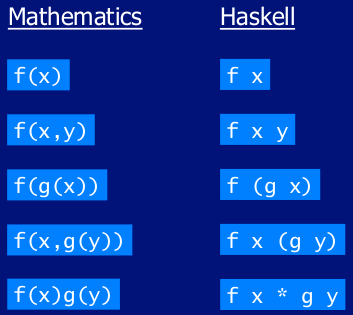
\includegraphics[width=0.3\textwidth]{figures/haskellMath.png}
\caption{Examples}
\end{figure}

\hypertarget{haskell-scripts}{%
\subsubsection{Haskell Scripts}\label{haskell-scripts}}

\begin{itemize}
\tightlist
\item
  New functions are defined within a script, a text file comprising a
  sequence of definitions
\item
  By convention, Haskell scripts usually have a .hs suffix on their
  filename. This is not mandatory, but is useful for identification
  purposes
\item
  To start a script, type in ghci test.hs (test.hs is the script name)
\item
  To use commands within the script, one can type `command-name`
\end{itemize}

\begin{lstlisting}[language=Haskell]
average ns = sum ns `div` length ns
\end{lstlisting}

\clearpage